\documentclass[11pt,]{article}
\usepackage{lmodern}
\usepackage{amssymb,amsmath}
\usepackage{ifxetex,ifluatex}
\usepackage{fixltx2e} % provides \textsubscript
\ifnum 0\ifxetex 1\fi\ifluatex 1\fi=0 % if pdftex
  \usepackage[T1]{fontenc}
  \usepackage[utf8]{inputenc}
\else % if luatex or xelatex
  \ifxetex
    \usepackage{mathspec}
  \else
    \usepackage{fontspec}
  \fi
  \defaultfontfeatures{Ligatures=TeX,Scale=MatchLowercase}
\fi
% use upquote if available, for straight quotes in verbatim environments
\IfFileExists{upquote.sty}{\usepackage{upquote}}{}
% use microtype if available
\IfFileExists{microtype.sty}{%
\usepackage{microtype}
\UseMicrotypeSet[protrusion]{basicmath} % disable protrusion for tt fonts
}{}
\usepackage[margin=1in]{geometry}
\usepackage{hyperref}
\hypersetup{unicode=true,
            pdftitle={A User-Friendly U.S. Census Browser for R},
            pdfauthor={Kiegan Rice},
            pdfborder={0 0 0},
            breaklinks=true}
\urlstyle{same}  % don't use monospace font for urls
\usepackage{color}
\usepackage{fancyvrb}
\newcommand{\VerbBar}{|}
\newcommand{\VERB}{\Verb[commandchars=\\\{\}]}
\DefineVerbatimEnvironment{Highlighting}{Verbatim}{commandchars=\\\{\}}
% Add ',fontsize=\small' for more characters per line
\usepackage{framed}
\definecolor{shadecolor}{RGB}{248,248,248}
\newenvironment{Shaded}{\begin{snugshade}}{\end{snugshade}}
\newcommand{\KeywordTok}[1]{\textcolor[rgb]{0.13,0.29,0.53}{\textbf{{#1}}}}
\newcommand{\DataTypeTok}[1]{\textcolor[rgb]{0.13,0.29,0.53}{{#1}}}
\newcommand{\DecValTok}[1]{\textcolor[rgb]{0.00,0.00,0.81}{{#1}}}
\newcommand{\BaseNTok}[1]{\textcolor[rgb]{0.00,0.00,0.81}{{#1}}}
\newcommand{\FloatTok}[1]{\textcolor[rgb]{0.00,0.00,0.81}{{#1}}}
\newcommand{\ConstantTok}[1]{\textcolor[rgb]{0.00,0.00,0.00}{{#1}}}
\newcommand{\CharTok}[1]{\textcolor[rgb]{0.31,0.60,0.02}{{#1}}}
\newcommand{\SpecialCharTok}[1]{\textcolor[rgb]{0.00,0.00,0.00}{{#1}}}
\newcommand{\StringTok}[1]{\textcolor[rgb]{0.31,0.60,0.02}{{#1}}}
\newcommand{\VerbatimStringTok}[1]{\textcolor[rgb]{0.31,0.60,0.02}{{#1}}}
\newcommand{\SpecialStringTok}[1]{\textcolor[rgb]{0.31,0.60,0.02}{{#1}}}
\newcommand{\ImportTok}[1]{{#1}}
\newcommand{\CommentTok}[1]{\textcolor[rgb]{0.56,0.35,0.01}{\textit{{#1}}}}
\newcommand{\DocumentationTok}[1]{\textcolor[rgb]{0.56,0.35,0.01}{\textbf{\textit{{#1}}}}}
\newcommand{\AnnotationTok}[1]{\textcolor[rgb]{0.56,0.35,0.01}{\textbf{\textit{{#1}}}}}
\newcommand{\CommentVarTok}[1]{\textcolor[rgb]{0.56,0.35,0.01}{\textbf{\textit{{#1}}}}}
\newcommand{\OtherTok}[1]{\textcolor[rgb]{0.56,0.35,0.01}{{#1}}}
\newcommand{\FunctionTok}[1]{\textcolor[rgb]{0.00,0.00,0.00}{{#1}}}
\newcommand{\VariableTok}[1]{\textcolor[rgb]{0.00,0.00,0.00}{{#1}}}
\newcommand{\ControlFlowTok}[1]{\textcolor[rgb]{0.13,0.29,0.53}{\textbf{{#1}}}}
\newcommand{\OperatorTok}[1]{\textcolor[rgb]{0.81,0.36,0.00}{\textbf{{#1}}}}
\newcommand{\BuiltInTok}[1]{{#1}}
\newcommand{\ExtensionTok}[1]{{#1}}
\newcommand{\PreprocessorTok}[1]{\textcolor[rgb]{0.56,0.35,0.01}{\textit{{#1}}}}
\newcommand{\AttributeTok}[1]{\textcolor[rgb]{0.77,0.63,0.00}{{#1}}}
\newcommand{\RegionMarkerTok}[1]{{#1}}
\newcommand{\InformationTok}[1]{\textcolor[rgb]{0.56,0.35,0.01}{\textbf{\textit{{#1}}}}}
\newcommand{\WarningTok}[1]{\textcolor[rgb]{0.56,0.35,0.01}{\textbf{\textit{{#1}}}}}
\newcommand{\AlertTok}[1]{\textcolor[rgb]{0.94,0.16,0.16}{{#1}}}
\newcommand{\ErrorTok}[1]{\textcolor[rgb]{0.64,0.00,0.00}{\textbf{{#1}}}}
\newcommand{\NormalTok}[1]{{#1}}
\usepackage{graphicx,grffile}
\makeatletter
\def\maxwidth{\ifdim\Gin@nat@width>\linewidth\linewidth\else\Gin@nat@width\fi}
\def\maxheight{\ifdim\Gin@nat@height>\textheight\textheight\else\Gin@nat@height\fi}
\makeatother
% Scale images if necessary, so that they will not overflow the page
% margins by default, and it is still possible to overwrite the defaults
% using explicit options in \includegraphics[width, height, ...]{}
\setkeys{Gin}{width=\maxwidth,height=\maxheight,keepaspectratio}
\IfFileExists{parskip.sty}{%
\usepackage{parskip}
}{% else
\setlength{\parindent}{0pt}
\setlength{\parskip}{6pt plus 2pt minus 1pt}
}
\setlength{\emergencystretch}{3em}  % prevent overfull lines
\providecommand{\tightlist}{%
  \setlength{\itemsep}{0pt}\setlength{\parskip}{0pt}}
\setcounter{secnumdepth}{5}
% Redefines (sub)paragraphs to behave more like sections
\ifx\paragraph\undefined\else
\let\oldparagraph\paragraph
\renewcommand{\paragraph}[1]{\oldparagraph{#1}\mbox{}}
\fi
\ifx\subparagraph\undefined\else
\let\oldsubparagraph\subparagraph
\renewcommand{\subparagraph}[1]{\oldsubparagraph{#1}\mbox{}}
\fi

%%% Use protect on footnotes to avoid problems with footnotes in titles
\let\rmarkdownfootnote\footnote%
\def\footnote{\protect\rmarkdownfootnote}

%%% Change title format to be more compact
\usepackage{titling}

% Create subtitle command for use in maketitle
\newcommand{\subtitle}[1]{
  \posttitle{
    \begin{center}\large#1\end{center}
    }
}

\setlength{\droptitle}{-2em}
  \title{A User-Friendly U.S. Census Browser for R}
  \pretitle{\vspace{\droptitle}\centering\huge}
  \posttitle{\par}
  \author{Kiegan Rice}
  \preauthor{\centering\large\emph}
  \postauthor{\par}
  \date{}
  \predate{}\postdate{}

\usepackage{float}

\begin{document}
\maketitle

\section{Introduction}

Census data is an important snapshot of information about a country at
different times throughout their history, one whose value is difficult
to overstate. While history books present a narrative of the events that
occured, students often don't get to interact with the raw data
themselves in that learning environment. Clean and accessible census
data allows the exploration of different demographic groups over time,
or investigations of a particular period of time and what the
demographic and economic landscape looked like in the past. Even today,
data about the world around us opens a pathway for learning more about
places we haven't been and groups of people we may not usually engage
with.

From an early point in the United States' history, there were many
``eminent men of science'' who recognized the value of the census data
and worked to aggregate and present the data that had been collected on
the population. Francis A. Walker's ``Statistical Atlas of the United
States'', based on the 1870 census, was an impressive effort in
aggregating population data to present it in a visually appealing way.
Although the Census Bureau's ``Statistical Atlases'' eventually stopped
being made, they were an important start to the effort of visually
presenting census data to a wider public.

Today, as methods of data analysis and visualization continue to be
developed and improved, access to census data allows us to look back on
that history and explore, synthesize, and visualize the information.
When aggregated and presented in a clear manner, viewers can learn more
about patterns in many different parts of the population.

\emph{Mention Dr.~Hofmann's paper on recreating/improving the
Statistical Atlas here\ldots{} forthcoming? published? As well as
Haley's ggmosaic stuff.}

Ever-improving visualization and data-wrangling methods in R (R Core
Team 2015) give those interested in statistical graphics a wealth of
opportunities to explore and learn from data; in particular,
incorporating user interactivity using Shiny has revolutionized the way
statisticians share and communicate information (Chang et al. 2017).
However, it is difficult to make use of these tools on census data if
that data is not available and easy to explore in one location.

An inherent problem in census data is that a country's census changes
over time; the variables collected, how they are collected, and even the
locations they are collected on are updated as the country is formed,
and subsequently grows and changes. The United States census data is no
exception to this rule. In a little under two and a half centuries, the
census has taken on many different forms. Data on occupations has
transformed as the employment landscape has changed; new states have
been formed, the most recent being within the last 100 years;
definitions of various demographic groups and the terminology used to
describe them have been updated as the demographic makeup of the country
has changed. Each decennial census brings a different set of variables
to the table. Sometimes these variables are new things the Census Bureau
is interested in learning about, while sometimes they remove variables
that are no longer relevant or whose information is captured somewhere
else.

Unfortunately, because the founders of the U.S. Census were unable see
200 years into the future, those interested in working with census data
are left with quite the inescapable mess. If you want to focus in on a
particular demographic group and their journey as part of the population
of the United States, you may have ten or more different variables names
to describe that one group over the course of the census from 1790 to
1960 - and that is just for one single group! Of course, we cannot just
simply change variable names to match our own research needs. It is
important to keep the data in its true form and be honest to the way
that the population was defined at different times throughout history,
even if our instinct may be to `clean' the data by changing variable
names.

This, of course, leaves the user with a wide variety of variables that
are far from consistent across years. In order to track one demographic
group across years - let alone many groups - a clean user interface that
helps users see exactly what information is available to them is a
necessity. To streamline the process and assist researchers in finding
out what information they have access to and what information they lack,
a U.S. Census Browser for R is presented, with the user interface being
a Shiny application, and the downloadable files being `tidy' csv files
that those with a small amount of R experience should be able to work
with.

\section{Background (Literature Review?)}

There are two main datasets that contain the aggregated counts of
historical, demographic, economic, and social characteristics from the
United States decennial census. They were both collected and developed
by the Inter-University Consortium for Political and Social Research.
The ICPSR 3, gathered from computer-readable data collections from the
U.S. Census Bureau as well as other reports (both published and
unpublished), contains data from 1790 to 1960. The ICPSR 2896, including
much of the same information as the ICPSR 3, also includes a wider array
of variables including manufacturing, and more county and city-level
information. The ICPSR 2896 as a dataset is a restricted access dataset
and requires users be part of a member institution in order to gain
access to it.

The University of Virginia Library hosted a ``Historical Census
Browser'' for many years that allowed users to search United States
Decennial Census Data for use in research, teaching, and personal
inquiry (Virginia Library 2017). The data included records on various
aspects of the U.S. population from the 1790 Census through the 1960
Census, originally populated using the ICPSR 3 dataset. This Historical
Census Browser was free and available for use for anyone with an
internet connection. The browser allowed a user to peruse available
topics for each census year, at both the state and county levels. The
Historical Census Browser was taken down on December 31, 2016, with the
county-level aggregated data becoming unavailable several months before
this. The source was widely used, with several other university
libraries and educational resources including University of California
Santa Barbara (California Santa Barbara Library 2010), University of
Pennsylvania (Pennsylvania Population Studies Center 2017), University
of Michigan (University of Michigan Population Studies Center 2017), and
the Smithsonian's History Explorer (American History 2008) directing
researchers to use the University of Virginia site as of 2017.

The University of Virginia Libraries website now directs users to Social
Explorer or the National Historical Geographic Information System
(NHGIS) website. Social Explorer, populated with the ICPSR 2896 data,
requires that users pay to use (or use through paid library access), and
does not offer a complete download of information. NHGIS, hosted through
the University of Minnesota, is very difficult for users to navigate
when looking for specific information across multiple years. The
Integrated Public Use Microdata Series (IPUMS USA), also hosted by the
University of Minnesota, gives microsamples of census data on a finer
grid - by person and household. However, this lacks state-aggregated
data. The Institute for Social Research at the University of Michigan,
which hosts the Inter-university Consortium for Political and Social
Research (ICPSR) database, has both the full ICPSR 2896 dataset and the
full ICPSR 3 dataset. Each of these are split into a separate data set
for each year and by split by county-level and state-level. This
database requires that users be a part of a member institution, and
requires users to agree that they will not distribute the information in
any way after gaining access to it. It also does not have any browser
function for users to look at the data - they must download the file for
each year, in either a SAS, SPSS, ASCII, or Stata set-up.

None of the aforementioned resources provide the full advantages that
the Historical Census Browser offered: a free-to-use and user-friendly
data browser that allows users to choose which data they are interested
in using, and download the complete aggregated records for their own
independent use. Having the data provided by the Historical Census
Browser available once again and streamlined for simple and easy data
browsing is a valuable resource for researchers and others alike.

\section{Work}

\subsection{Data}

Although the county-level data had already been removed from the
website, the state-level aggregated records for each decennial census
from 1790 through 1960 were captured from the website in September of
2016 and saved as raw data with the intent to create a resource for R
users that allowed the same main functionalities of the original
University of Virginia Historical Census Browser, streamlined for easy
data searches and data management.

The majority of files for the decennial censuses were complete upon
capture from the website. However, two years of census data were missing
some column names and thus needed to be verified. For the 1890 and 1940
censuses, each column was compared to all columns from ICPSR 2896 and
ICPSR 3 data files by both correlation and Euclidean distance, and thus
some columns were able to be correctly identified.

\emph{Describe this process in more detail once I actually get this
figured. How many columns were correctly matched? How many weren't?}

\emph{Currently I am struggling with the available data formats from
ICPSR. I was able to compare the ICPSR 2896, but not many of the
variables were actually able to be matched up, and I suspect this is
because the ICPSR 2896 has some different values than the ICPSR 3. The
ICPSR 3 is looking much more promising for verifying the column names,
but\ldots{} it doesn't give column names. I have the variable names in a
codebook, but I am stuck between manually entering in all of the column
names (there are 259 of them) and finding an overly complicated way to
automate that processs\ldots{}}

Each year of the dataset began in a separate file, with each row
corresponding to a State, each column being a demographic variable, and
values being state-aggregated counts of number of people in that
category. Each state was given a label \texttt{Type} as either a State
or Territory, as some U.S. territories participated in the decennial
census before they received full statehood. Each individual file can be
found as \texttt{states} followed by the year of the census, (e.g.
\texttt{states1790}) in this package. Each of these datasets were
combined into one list, \texttt{stateslist}, which is the list of data
that is used to populate the census browser.

\subsection{Description}

This package includes the state-aggregated data for each individual
year, as well as a list of all of the years together. The intended
interaction with these data sources is via the Shiny application,
\texttt{Get\ Your\ Data}. This interactive Shiny application presents
the user with two options - focusing on a single year of the census,
found in the \texttt{Single\ Year} tab, or focusing on multiple years at
once, found in the \texttt{Multiple\ Years} tab.

The \texttt{Single\ Year} tab allows users to choose which year they are
interested in from a drop-down menu, as well as two manual search entry
boxes for variables of interest. For example, if a user is interested in
the prevalence of farms in 1860, they can select 1860 and then search
for ``farms'' in the first ``Variable of Interest'' spot (see Figure 1).
Users can then see a complete list of all variable names in that
particular year that have ``farms'' in their title. With this list now
available, users can select each variable they want by clicking on it.
Once all desired variables have been selected, clicking on the
``Download Filtered Data'' button will open a window in which the user
can choose a file name and directory location for saving the resulting
comma-separated values file. Variables will not remain selected if the
user chooses to change their search term or add a second search term.
However, if the user has interest in many separate variables that
require different search terms, it is quite easy to combine multiple csv
files in R using \texttt{full\_join} from the \texttt{dplyr} package and
specifying \texttt{State}, \texttt{Year}, \texttt{TOTAL.POPULATION}, and
\texttt{Type} as the variables to join by. These four variables will
always be included in the resulting csv file, whether the user selects
them or not.

\begin{figure}[htbp]
\centering
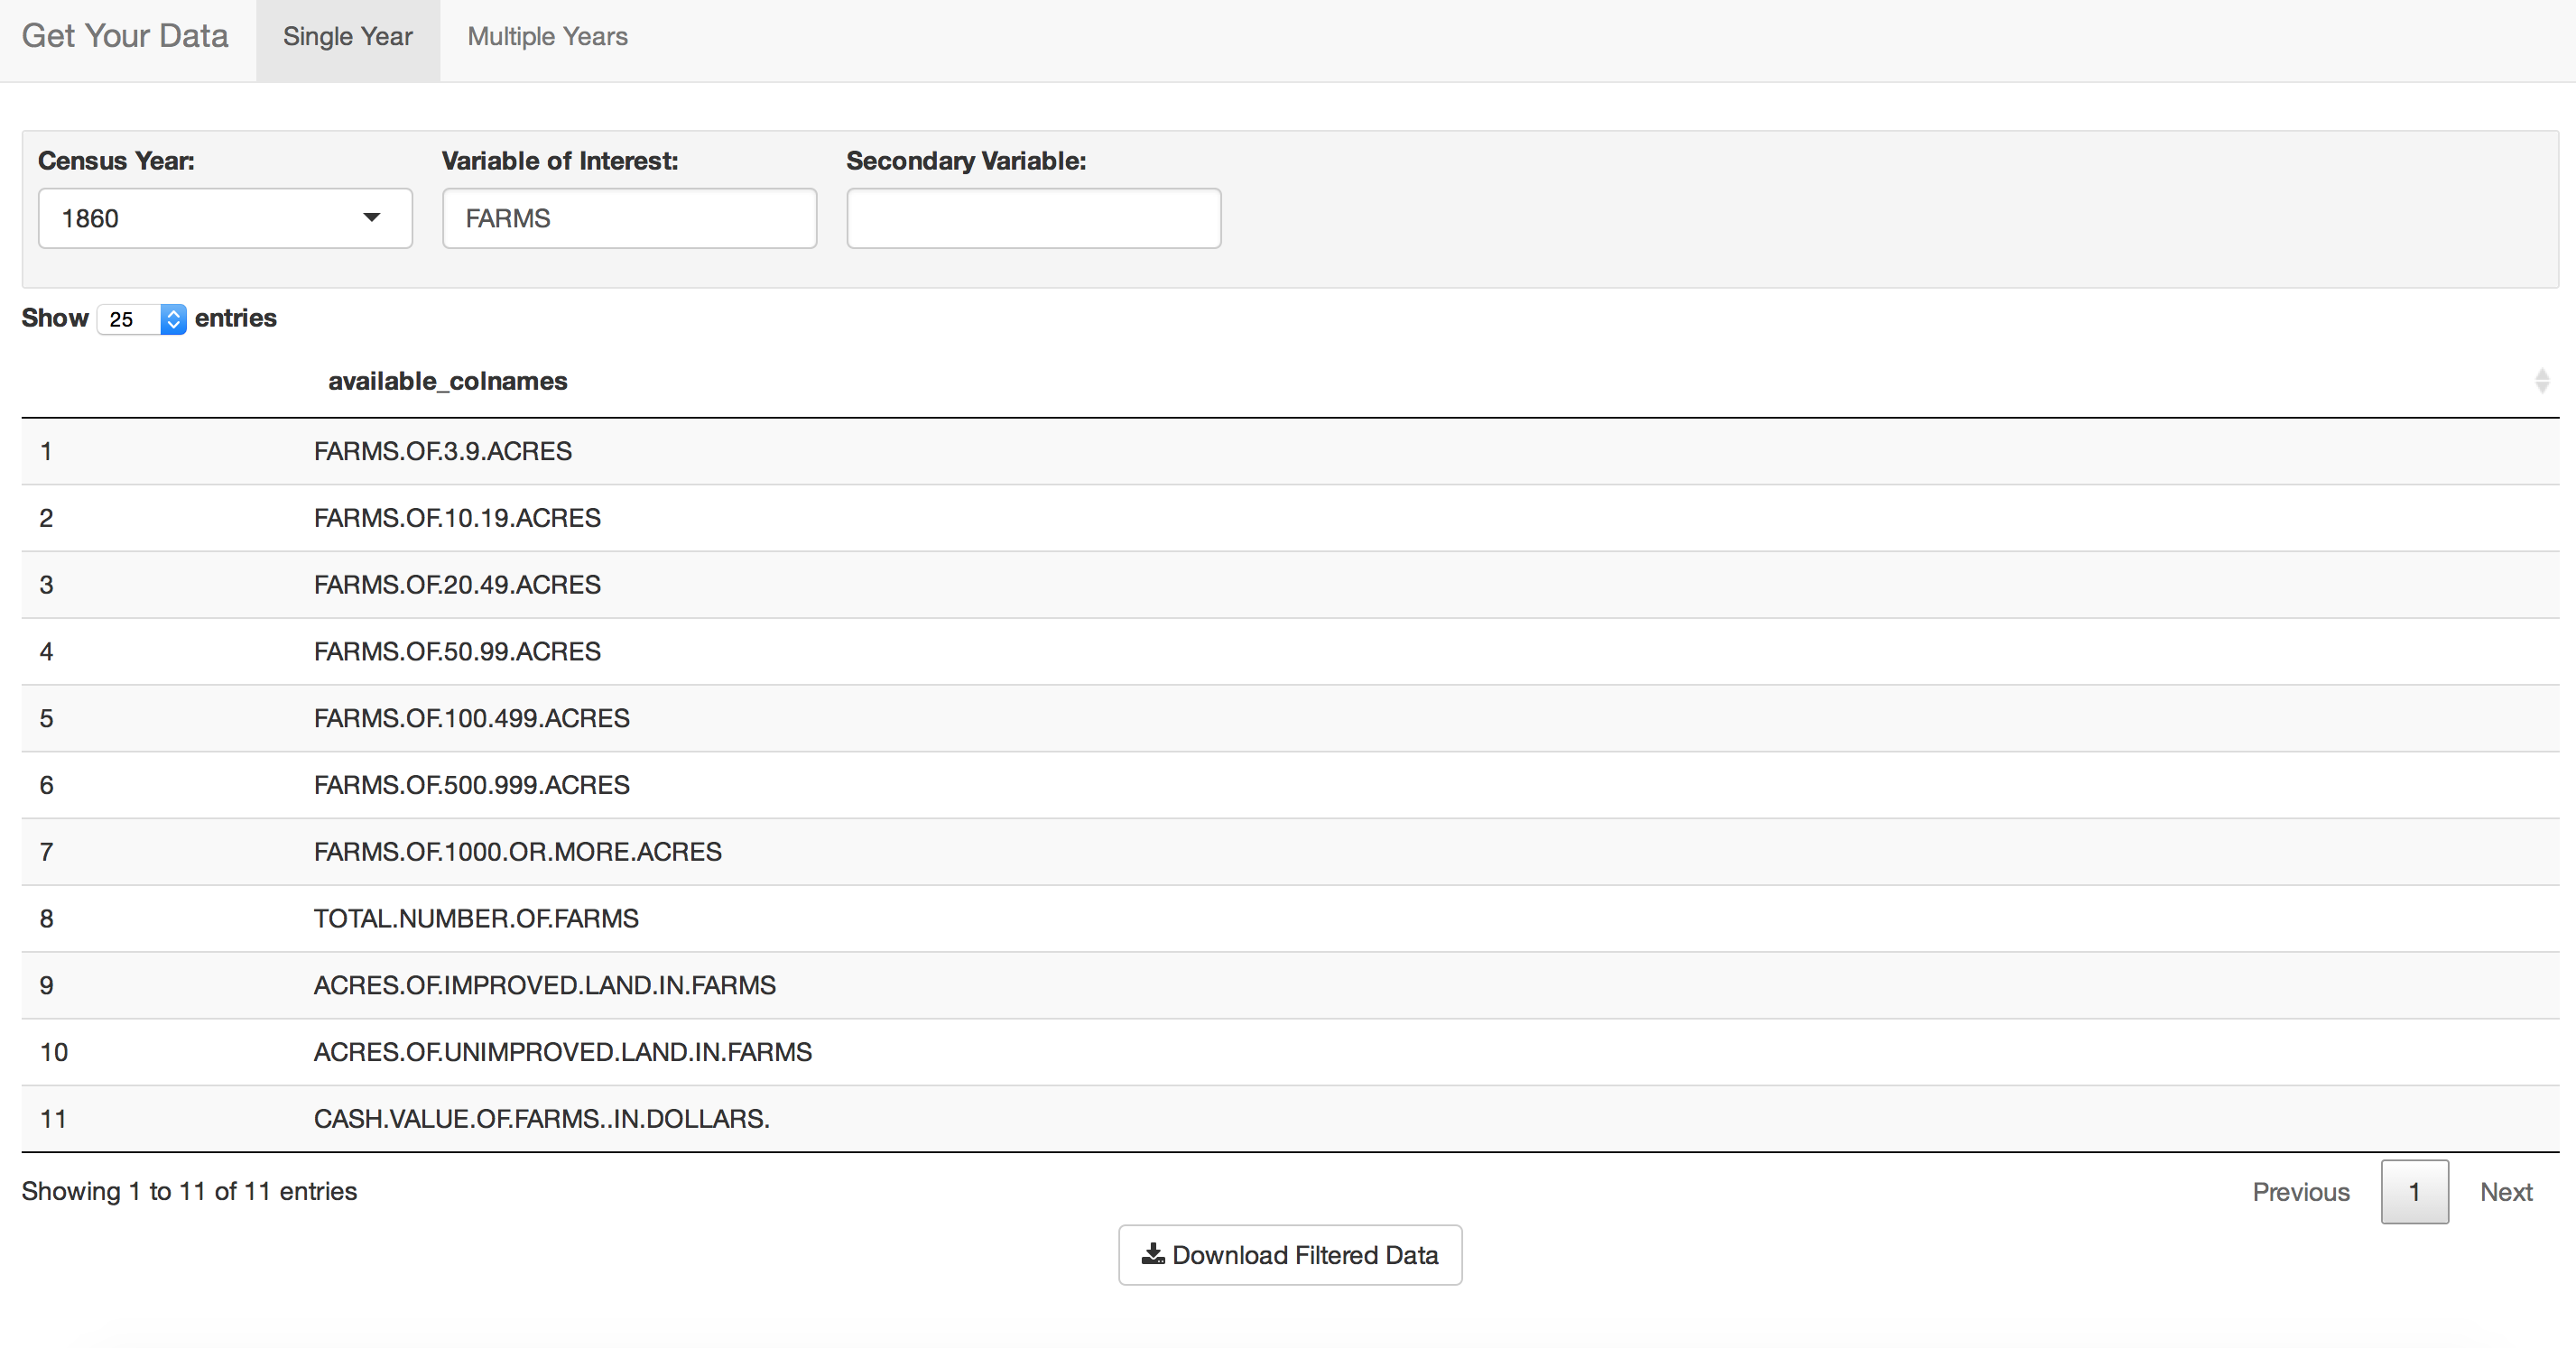
\includegraphics{./figures/app-sshot-farms.png}
\caption{The resulting view of a search for farms in the 1860 U.S.
Census on the \texttt{Single\ Year} tab of the \texttt{Get\ Your\ Data}
app.}
\end{figure}

The \texttt{Multiple\ Years} tab allows users to look for variables of
interest over a range of years. It offers all decennial censuses from
1790 to 1960, and offers the same search tool as before, but only allows
users to narrow down results by one search term rather than the two
provided in the \texttt{Single\ Year} tab. Users can select the range of
years they are interested in by using the slider tool to specify their
range of interest, and subsequently use the ``Variable of Interest''
search bar to narrow down their results. The results, being
two-dimensional rather than just a single list of available variables,
are presented somewhat differently in the \texttt{Multiple\ Years} tab.
Each available variable is listed along the left side of the interface,
and each selected year is presented across the top as a column in the
table (see Figure 2). For each variable in the table, an \texttt{X}
indicates for which years that particular variable is present. Far to
the right, there is a column which denotes a count how many of the
selected years have that particular variable. Users can choose to order
the results by most years present to least years present, if they
choose. This is where it is important to keep in mind that variable
names for different demographic groups change drastically over the
course of the decennial census, and thus users will want to be cognizant
of varying search terms that may need to be checked. \emph{Should I
still try to add a feature that pops up when they look for certain
search terms? This seems hard to do without singling out a few groups,
since pretty much every group has changed terminologies over time.}

Similar to the output file of the \texttt{Single\ Year} tab, once a user
selects all variables they are interested in, they can select the
``Download Filtered Data'' button to download a csv file of the chosen
variables for all states across the selected years. For years in the
selected range that don't have a particular variable, the csv file will
be filled in with \texttt{NA} values, which allows the structure of the
data table to remain intact although there are some year-variable
combinations that do not exist in the data. As mentioned previously,
because of the changing nature of variable names in the decennial
census, users may have to search for several separate terms, download
each file separately, and combine them once the files are downloaded.
This process can be done in the same manner as the combination However,
they are fairly easy to combine because the structure ensures that key
variables needed to add on new columns are in place, regardless of which
variables users choose to download. This results in all information
about all variables of interest across the years of interest being
together in one data table, with each row representing a year-state
combination and all variables of interest represented as columns. Users
can easily filter on specific variables or years while still maintaining
the original full data set, which is advantageous for visualizing how a
demographic group changes over time.

\subsection{Example}

The \texttt{Get\ Your\ Data} Shiny app can be easily used to search for
a topic, find the data of interest, download state-level information,
and tell a visual story of populations in the United States over time.
To demonstrate the utility of this Shiny app, we will walk through an
example on the history of the African American population in the United
States. We begin by running the Shiny app:

\begin{Shaded}
\begin{Highlighting}[]
\KeywordTok{library}\NormalTok{(shiny)}
\NormalTok{shiny::}\KeywordTok{runGitHub}\NormalTok{(}\StringTok{"kiegan/censusbrowseR"}\NormalTok{, }\DataTypeTok{subdir =} \StringTok{"shiny"}\NormalTok{)}
\end{Highlighting}
\end{Shaded}

The default set of years is 1790 to 1880. However, the slider range can
be expanded to be able to explore data across all the available years.

\begin{figure}[htbp]
\centering
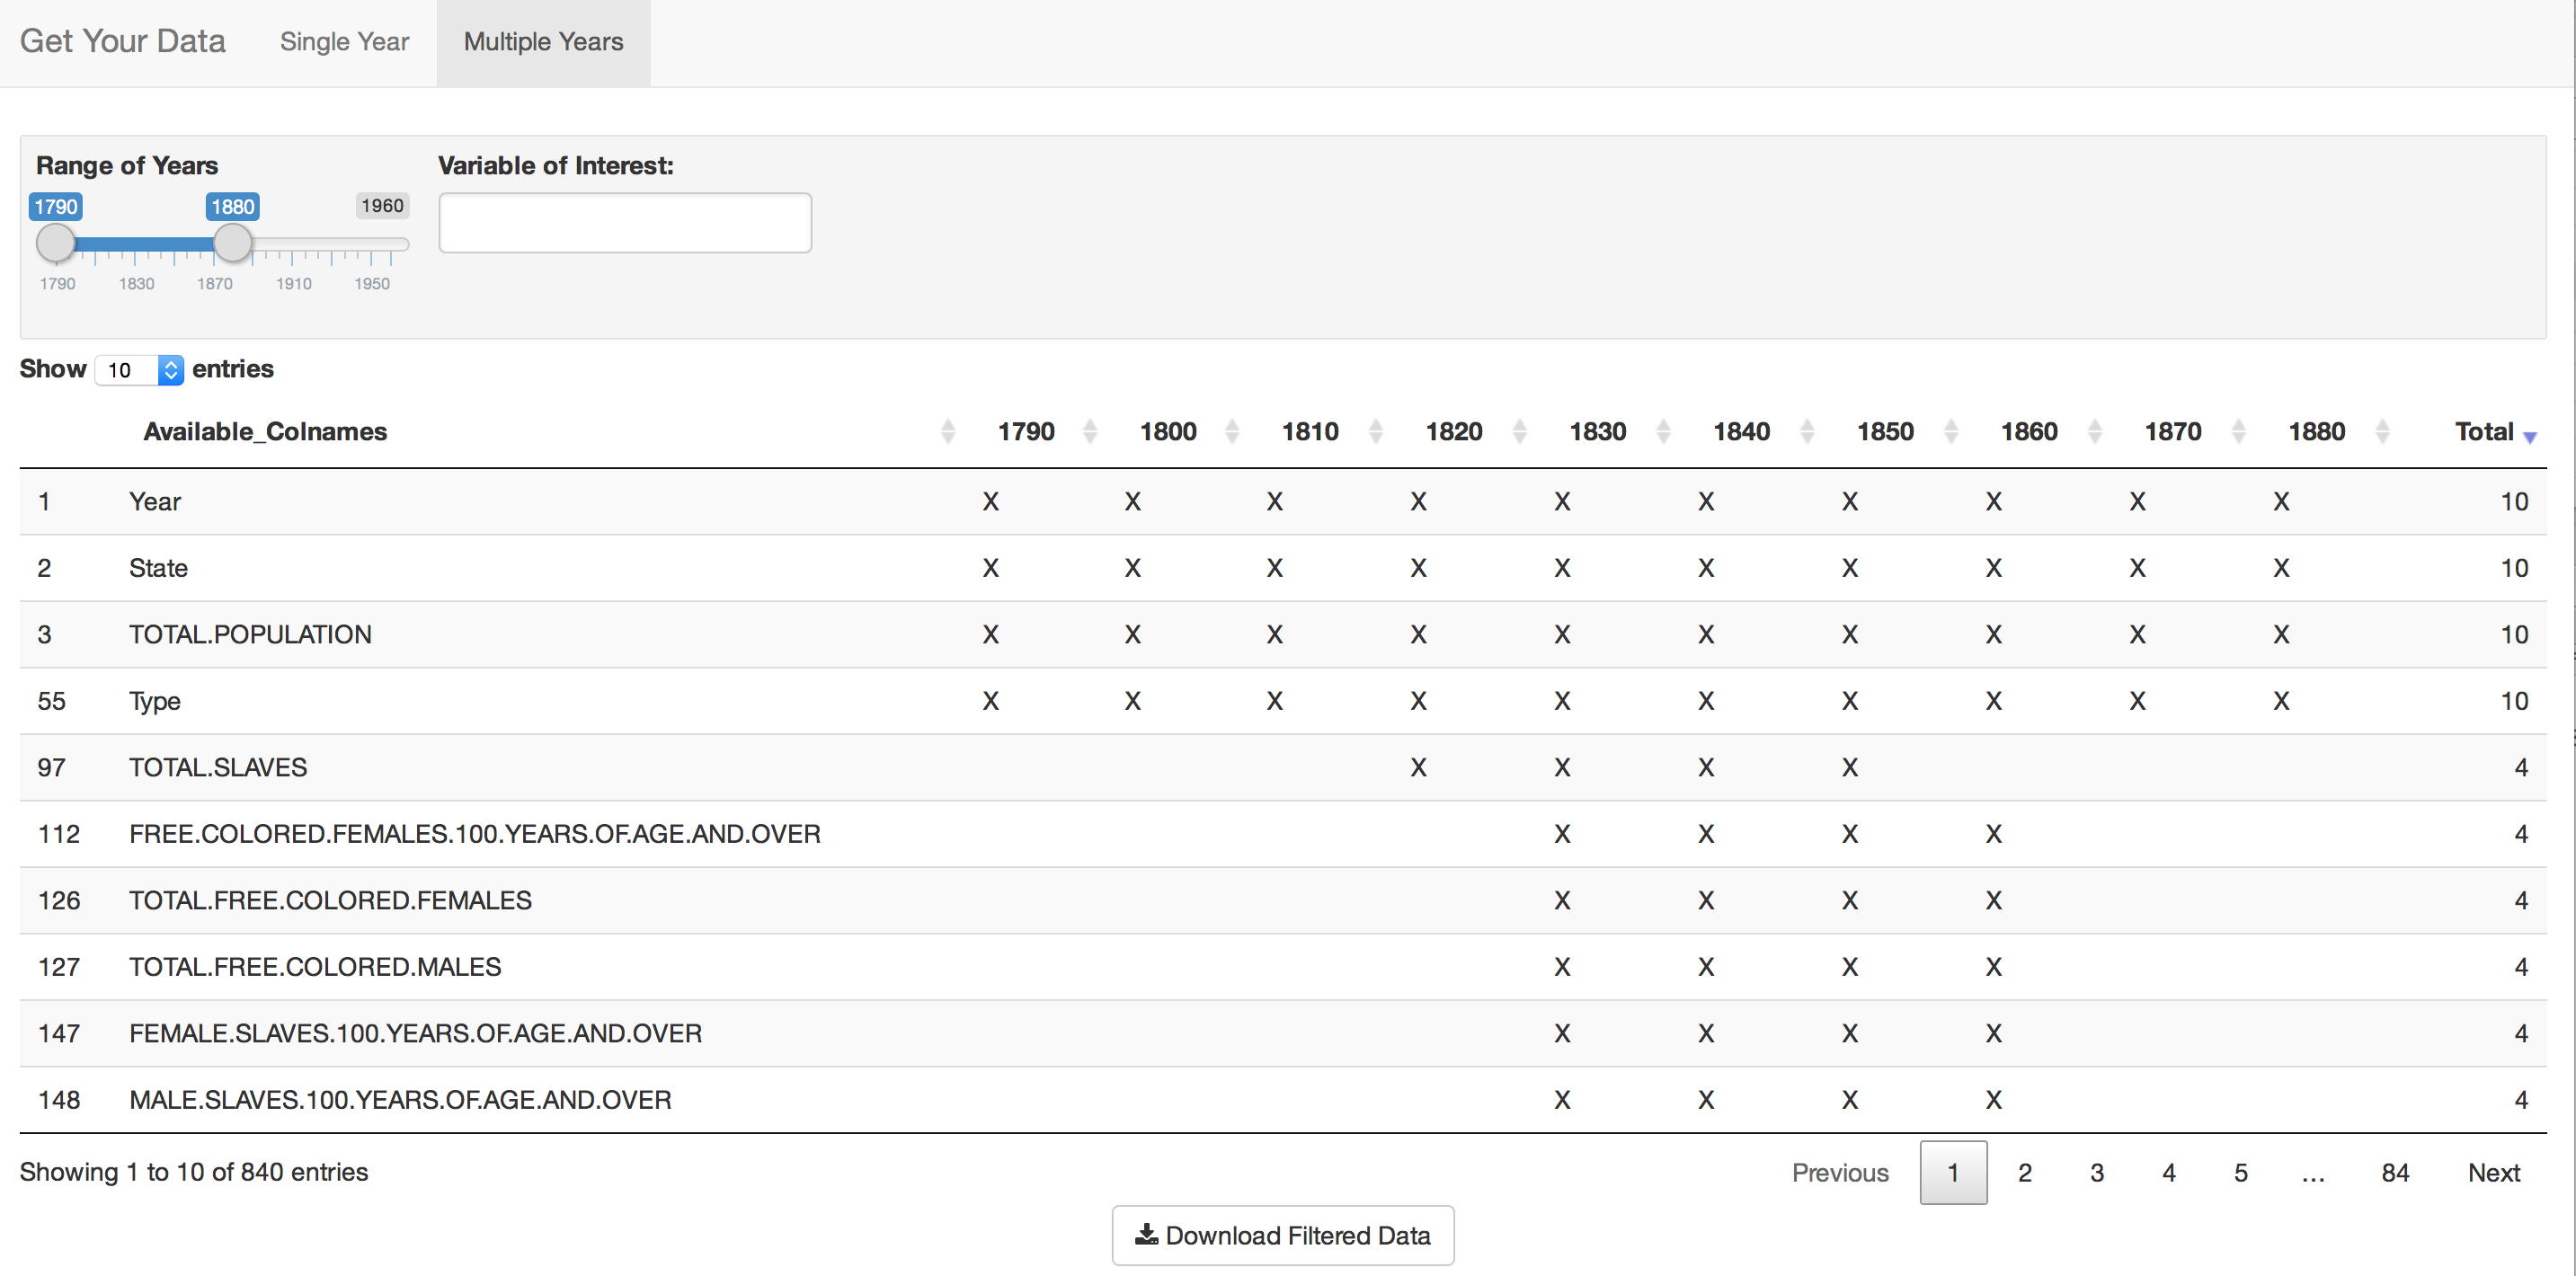
\includegraphics{./figures/app-sshot-multiple-years.png}
\caption{An example of available column names for the years 1790 to
1880.}
\end{figure}

After ordering by how many years they appear in, the available variable
names show a serious lack of continuity. The four ever-present variables
(\texttt{Year}, \texttt{State}, \texttt{TOTAL.POPULATION}, and
\texttt{Type}) each appear ten times, once in each year selected. After
that, the next most common variable only appears in four of the ten
years we have chosen. That immediately demonstrates some pretty
significant hurdles that will persist when tracking any demographic
group over time, without even focusing in on a particular group yet.

Since the focus is on African Americans throughout U.S. history, the
first search term needed is \texttt{SLAVE} in the early years of the
U.S. census. The vast majority of African Americans were slaves when the
United States was founded, so variables that count the number of slaves
are important variables to have in order to get a grasp on the African
American population in early U.S. history. It is important to note that
the \texttt{SLAVE} categorization is the only term the U.S. census had
related to African Americans in the early years of the census, so it is
also the only source of information available on that groupfor that time
period.

Once a relevant range of years has been chosen, we simply enter a search
term. Searching for \texttt{SLAVE} gives a list of all the possible
variable names across all years, which can again be sorted by how how
many years each variable name appears in. The results of this search can
be seen in Figure 3.

\begin{figure}[htbp]
\centering
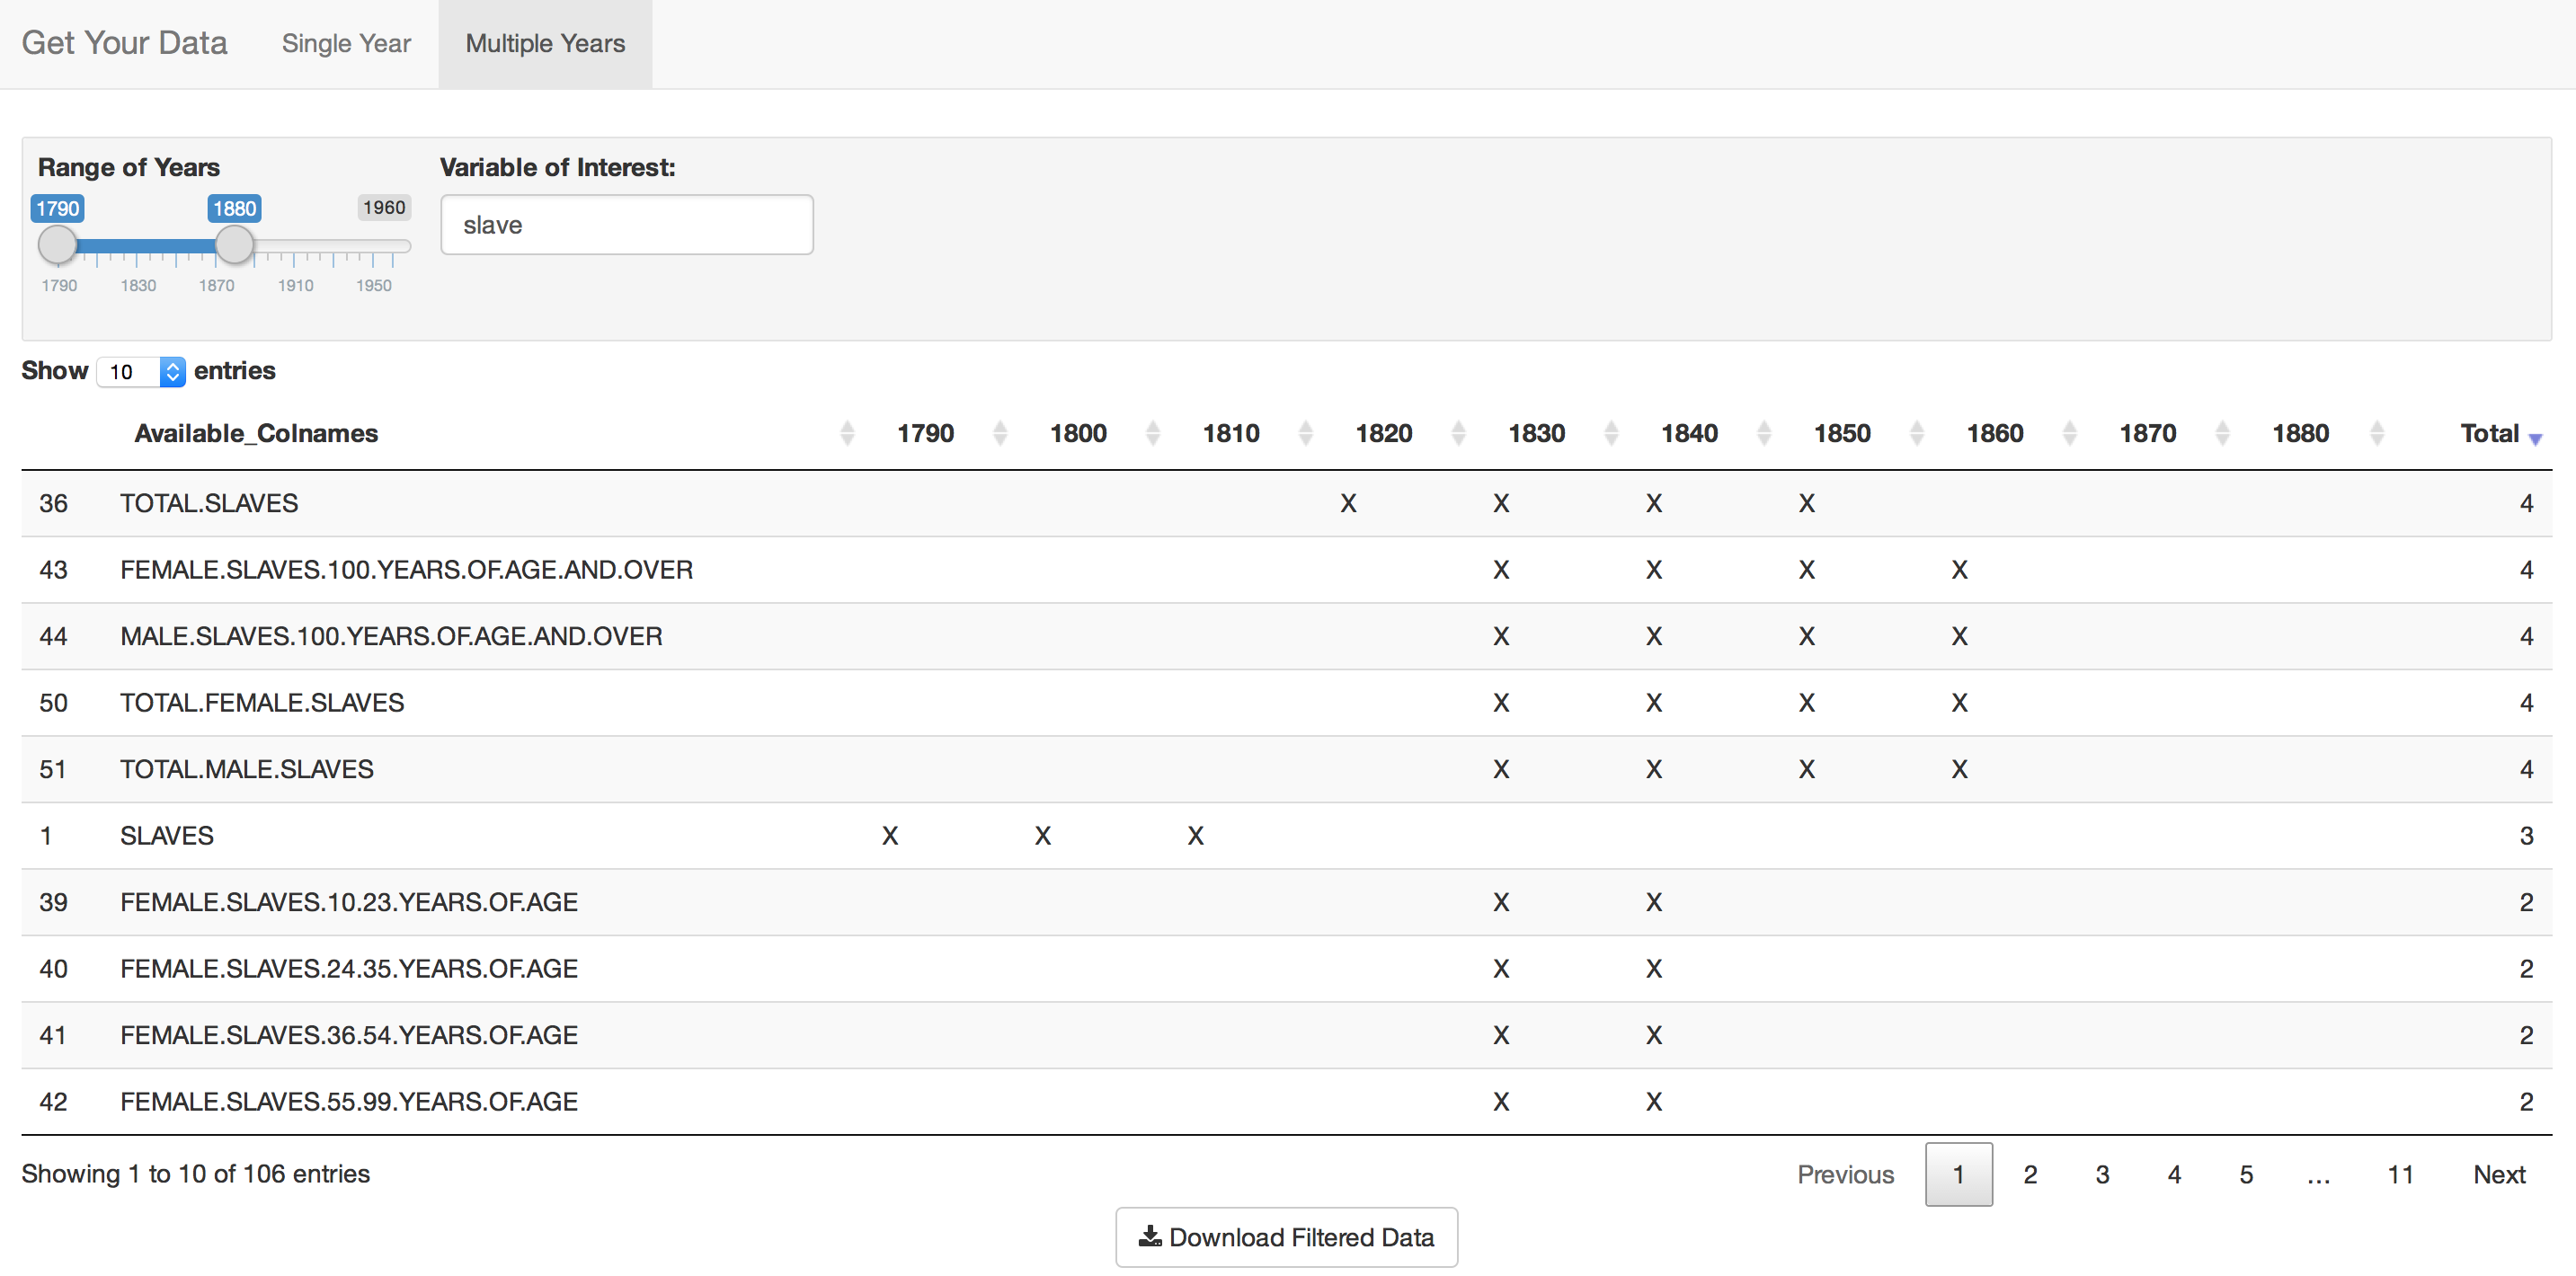
\includegraphics{./figures/app-sshot-slave.png}
\caption{The resulting table after searching for the term `slave' in the
\texttt{Get\ Your\ Data} app.}
\end{figure}

For this example, three separate searches were executed within the
\texttt{Get\ Your\ Data} app, using three different terms that the
census used to categorize African Americans at different points in the
decennial census (``slave'', ``colored'', and ``negro''). The third of
these terms, when used in plotting, will be labeled as ``black'' for the
remainder. This gave three separate csv files, which were easily
combined using \texttt{full\_join} from the \texttt{dplyr} package. Now,
for this demographic group, all of the state-aggregated population
counts are together in one data frame, although different terms are used
at different points in time.

The data, being combined, can now be explored. For any particular year,
a subset of the total dataset can be taken to include only information
for that year, for quicker determination of which variables are
available for that particular year. For example, after subsetting on the
year 1790, state-level counts of the \texttt{SLAVES} variable for that
year can be plotted. Use of the \texttt{USAboundaries} package in
concert with this census browser is recommended, as it provides the most
accurate boundaries of the United States at any given date (Mullen and
Bratt 2017). Just as variable names and the make-up of the census
rapidly changed throughout the United States' history, the boundaries of
the states and territories changed as well. The recorded
state-aggregated values in the dataset are for the states as they were
during that census year, and thus sometimes include demographic counts
from areas that differ from the currently defined boundaries.

\begin{figure}[htbp]
\centering
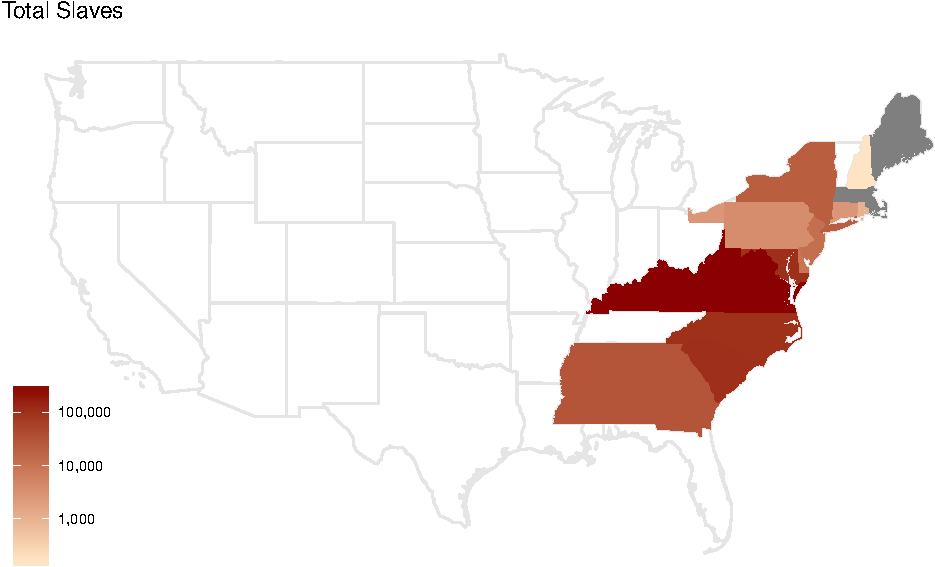
\includegraphics{writeup_files/figure-latex/chunk-1790-map-1.pdf}
\caption{Total number of slaves per state in 1790, plotted on a
continuous log scale. State boundaries for July 4, 1790 were gathered
from \texttt{USAboundaries} package.}
\end{figure}

Now, with a visualization of the slave population in the United States
in 1790 in hand, it is easy to look at subsequent years of the decennial
census in a similar manner to see how the population changes over time.

\begin{figure}[htbp]
\centering
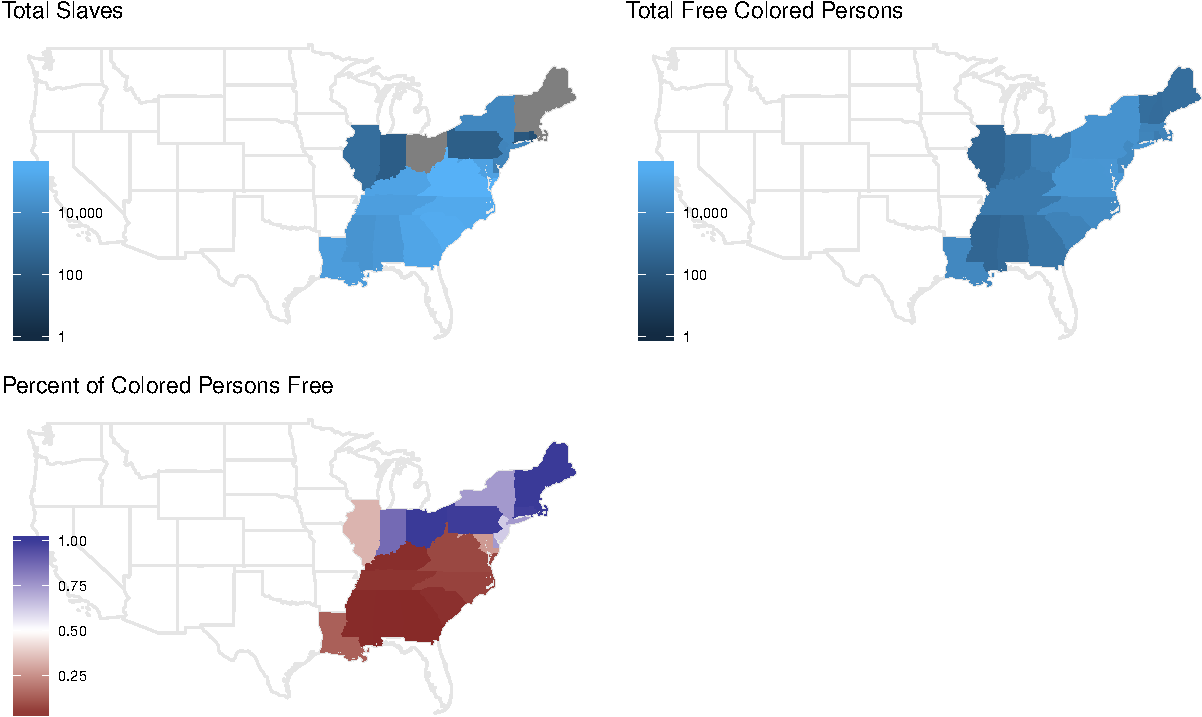
\includegraphics{writeup_files/figure-latex/unnamed-chunk-5-1.pdf}
\caption{Number of Slaves, Number of Free Colored Persons, and
Percentage of Free Colored Persons in 1820.}
\end{figure}

Jumping to the year 1820, and again filtering on that particular year,
we learn new information about the African American population. The
census at this time includes a count of
\texttt{TOTAL.FREE.COLORED.PERSONS}, as there are citizens who are
African American or other minorities that are free, and not slaves. At
this time, many minorities were grouped together in the ``colored
persons'' category, and as before, we do not have any other record for
African Americans except this categorization and the ``slaves''
categorization. However, since the 1820 census included records for both
\texttt{TOTAL.FREE.COLORED.PERSONS} and \texttt{TOTAL.SLAVES}, we can
also now visualize the percentage of African Americans in each state
that were categorized as ``free persons'' as opposed to slaves. Knowing
that both of these variables are available allows for a powerful
comparison by visualizing the growing divide in the United States at
that time.

\begin{figure}[htbp]
\centering
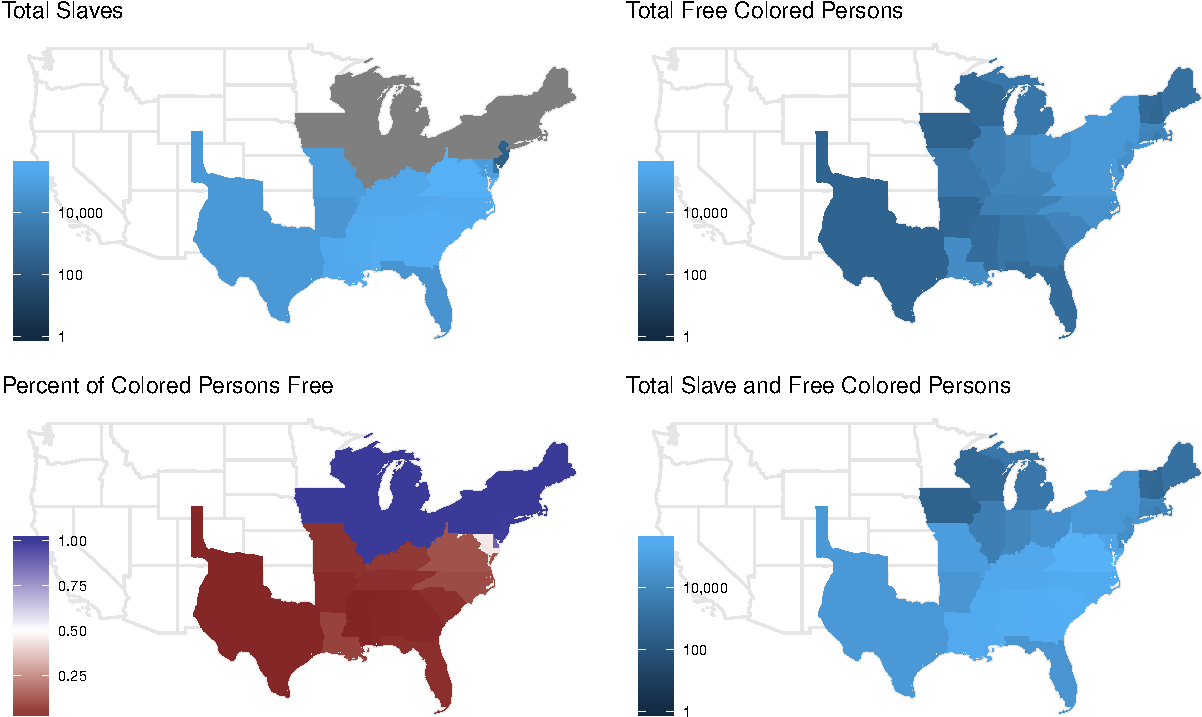
\includegraphics{writeup_files/figure-latex/unnamed-chunk-6-1.pdf}
\caption{Number of Slaves, Number of Free Colored Persons, Percentage of
Free Colored Persons, and Total African American Persons in 1850.}
\end{figure}

Moving forward from there, even more information can be gleaned about
this population. After subsetting on the year 1850, it is seen that
although there is still a \texttt{TOTAL.SLAVES} column in the record,
many states did not record this variable, as they were already free
states. We can transform these \texttt{NA} values into zeros to account
for this difference in the data and allow us to still calculate the
percentages of free African Americans. Starting in 1850, we can also
start investigating what the total African American population looks
like in each state, rather than just the slave population and free
population.

\begin{figure}[htbp]
\centering
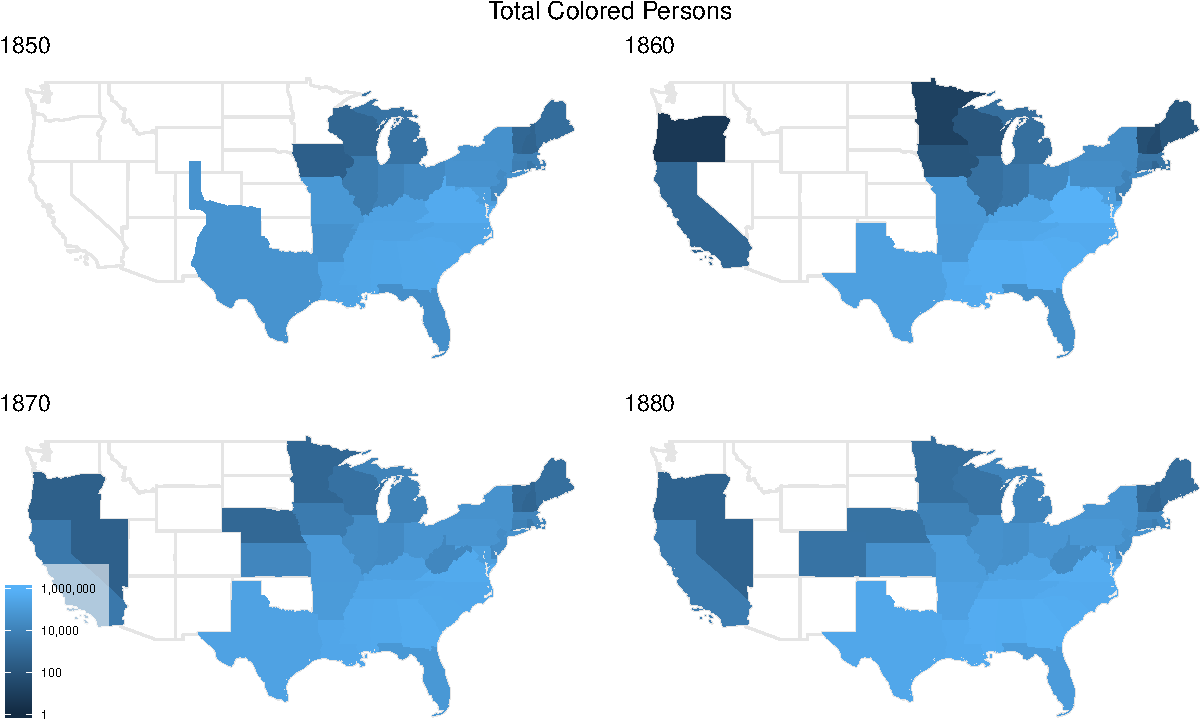
\includegraphics{writeup_files/figure-latex/unnamed-chunk-7-1.pdf}
\caption{Total Colored Persons in 19th Century United States}
\end{figure}

The total African American population is particularly interesting moving
forward as well after slavery is abolished in the 1860s and some
migration begins to occur out of certain areas. The balance of the total
African American population in each state begins to change somewhat as
the United States transitions into the post-slavery period. It is also
clear to see how the boundaries of states change and new states are
formed, with the United States gaining new states at each census.

\begin{figure}[htbp]
\centering
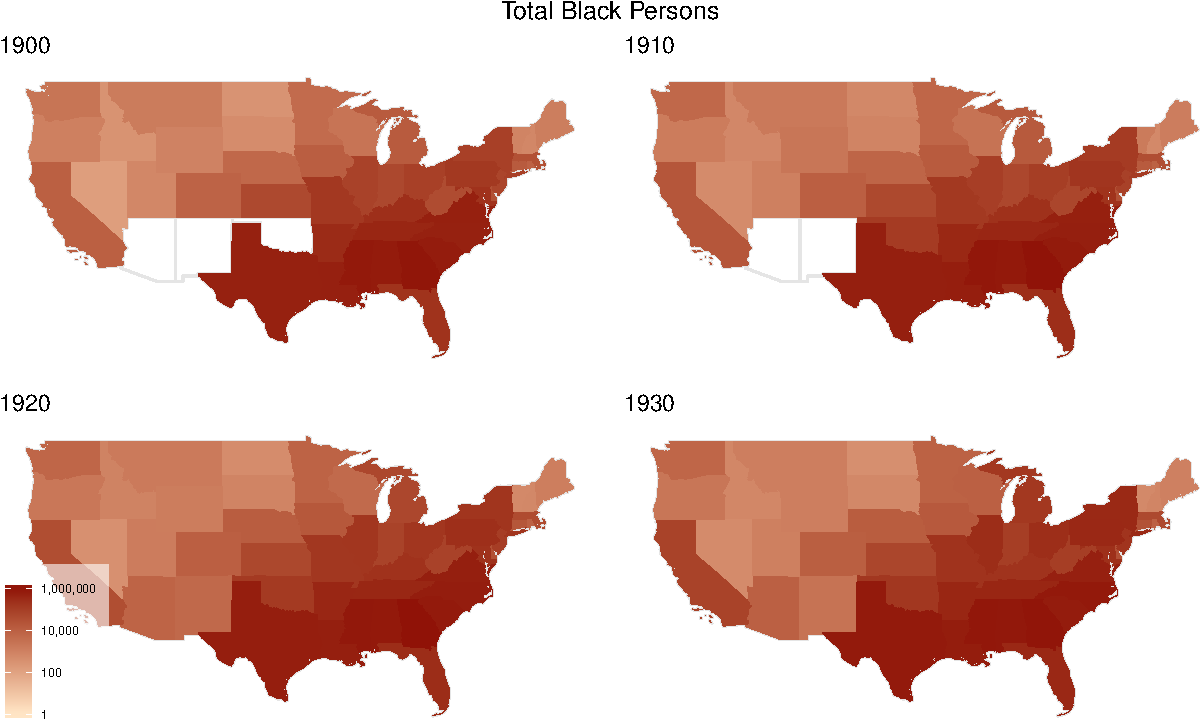
\includegraphics{writeup_files/figure-latex/unnamed-chunk-8-1.pdf}
\caption{Total Black Persons in 20th Century United States}
\end{figure}

A period of growth and change can be seen at the turn of the 20th
century as well, with a dramatic shift in the African American
population out west to California and with the balance in the east and
midwest shifting slightly further up north. Although the highest density
still remains in the southern states, somewhat of a northern migration
is visible.

\section{Discussion}

Although there is a lack of county-level data and the available data for
the census browser is only as recent as 1960, users are able to
efficiently find a group of interest at different points in U.S.
history, collect all of the relevant variables over time, and tell a
visual story about a growing nation and a changing population. This
connectivity across years and ability to assess what information was
available all in one browser demonstrates the time that could be saved
by researchers interested in delving into United States history.

As seen with the discrepancy in recording the \texttt{TOTAL.SLAVES}
variable in the 1850 census, the layout also assists in quicker
determination of not only which variables are available, but where
information is missing for some states on a particular variable. Finding
these differences is made much easier by having all relevant variables
in one data frame, which can be summarized and searched all at one time.

\section{Future Work}

In order to be able to investigate even more complex patterns in United
States history, having a finer grid of information - specifically
county-level data - would be extremely valuable. There are inherent
challenges with a more complex set of data such as county-level, which
promises lack of continuity across counties and states. Another big
challenge would be creating a carefully constructed layout in which
users can interact with not only years, but differences across locales
to find the most complete information. Despite these expected
challenges, adding county-level data to this browser would give
researchers a much richer resource to work with.

Just as there were many changes in the census between 1790 and 1960, the
census adapts and changes with each passing year. Different variables
are tracked, congressional boundaries change, and the demographic
landscape of the United States changes as well. Having current data
(through 2010) and being able to incorporate future data as it is
collected would allow for the juxtaposition of today's population with
that of the past. Being able to put history into context is an important
skill, and one that an up-to-date census browser could help facilitate
for students and researchers alike.

\section{References}

\hypertarget{refs}{}
\hypertarget{ref-SmithsonianHistoryExplorer}{}
American History, Smithsonian National Museum of. 2008. ``Smithsonian
History Explorer.''
\url{https://historyexplorer.si.edu/resource/historical-census-browser-university-virginia}.

\hypertarget{ref-UCSB-US-HCB}{}
California Santa Barbara Library, University of. 2010. ``United States
Historical Census Browser.''
\url{http://www.library.ucsb.edu/research/db/1304}.

\hypertarget{ref-Shiny}{}
Chang, W., J. Cheng, JJ. Allaire, Y. Xie, and J. McPherson. 2017.
``Shiny: Web Application Framework for R.'' Computer Program.
\url{http://CRAN.R-project.org/package=shiny}.

\hypertarget{ref-USAboundaries}{}
Mullen, L., and J. Bratt. 2017. ``USAboundaries: Historical and
Contemporary Boundaries of the United States of America.'' Computer
Program. \url{http://cran.r-project.org/web/packages/USAboundaries}.

\hypertarget{ref-UPenn-HCB}{}
Pennsylvania Population Studies Center, University of. 2017.
``Historical Census Browser - University of Virginia Library.'' Accessed
March 27.
\url{https://www.pop.upenn.edu/resource/historical-census-browser-university-virginia-library}.

\hypertarget{ref-RCoreTeam}{}
R Core Team. 2015. ``R: A Language and Environment for Statistical
Computing.'' Journal Article. \url{http://www.R-project.org}.

\hypertarget{ref-UMich-HCB}{}
University of Michigan Population Studies Center. 2017. ``Historical
Census Browser (1790 - 1960).'' Accessed March 27.
\url{http://www.psc.isr.umich.edu/dis/data/resource/detail/1369}.

\hypertarget{ref-HCB}{}
Virginia Library, University of. 2017. ``Historical Census Browser.''
\url{https://mapserver.lib.virginia.edu/}.


\end{document}
